\section{Channel Charting}
\label{sec:channel_charting}

Channel charting~\cite{studer2018channel_charting} aims to produce a
low-dimensional representation of the radio environment from CSI alone,
\emph{without} using UE position labels.
A good chart preserves the neighbourhood structure of the underlying
physical space: two UEs that are physically close should be mapped to
two chart points that are close, and vice versa.
This section applies four dimensionality-reduction (DR) methods to the
same $N=3\,186 \times D_f = 3690$ fingerprint matrix introduced in
Section~\ref{sec:localization} and benchmarks the resulting charts against
the $(x,y)$ ground truth using the metrics recommended in the channel-charting literature~\cite{studer2018channel_charting,lei2019siamese_cc}.

\subsection{Methods}

The following DR techniques are compared:
\begin{itemize}
  \item \textbf{PCA} --- linear principal-component projection, providing
        a best-case baseline for variance preservation.
  \item \textbf{t-SNE} --- non-linear stochastic neighbour embedding,
        parameterised by its perplexity~\cite{vandermaaten2008tsne}.
  \item \textbf{Autoencoder (AE)} --- a symmetric fully-connected
        encoder/decoder with a 2-D bottleneck, trained with an MSE
        reconstruction loss.
  \item \textbf{UMAP} --- uniform manifold approximation and projection,
        parameterised by its local neighbourhood size
        $n_{\mathrm{neighbors}}$~\cite{mcinnes2018umap}.
\end{itemize}
For t-SNE and UMAP the input is first reduced to 50~PCA components to
remove small-variance noise directions; this is the standard preprocessing
recommended by both method
authors~\cite{vandermaaten2008tsne,mcinnes2018umap}.
Perplexity (t-SNE) and $n_{\mathrm{neighbors}}$ (UMAP) are swept over
$\{5,15,30,50\}$ and $\{5,10,20,30\}$ respectively, and the best-scoring
configuration is retained.

t-SNE and UMAP are also implemented in MATLAB but without PCA reduction and applied to the \emph{tommiScene} dataset. 

\subsection{Metrics}

The chart is evaluated with four quality metrics, three of which are
label-free (they compare neighbourhood structures) and one of which uses
ground-truth positions as a reference:
\begin{itemize}
  \item \textbf{Trustworthiness (TW, $\uparrow$)}: penalises false
        neighbours -- points that look close in the chart but are far
        apart in the real RF space.
  \item \textbf{Continuity (CT, $\uparrow$)}: penalises tears -- points
        that are close in the real RF space but end up far apart in the
        chart.
  \item \textbf{Kolmogorov--Smirnov distance (KS, $\downarrow$)}: compares
        the chart's pairwise-distance distribution against the true
        geographic one.  $\text{KS}\to 0$ corresponds to a
        globally-scale-preserving chart.
  \item \textbf{Nearest-Neighbour Localization Error
        (NNLE, $\downarrow$, m)}: predicts the UE position by copying the
        coordinate of the chart's nearest neighbour and returns the mean
        Euclidean error.  This ties the chart quality back to a concrete
        downstream task.
\end{itemize}
An ideal chart satisfies $\text{TW}\approx\text{CT}\approx 1$,
$\text{KS}\approx 0$, and $\text{NNLE}$ on the order of the UE grid
spacing.

\subsection{Results}

Table~\ref{tab:cc_metrics} summarises the final scores, and
Fig.~\ref{fig:cc_x}--\ref{fig:cc_comparison} visualise the charts
coloured by the ground-truth $x$, $y$, and radial coordinates.

\begin{table}[htbp]
\caption{Channel-charting metrics on the Otaniemi\_small fingerprint
         matrix ($N=3\,186$).  Best value per column in \textbf{bold}.}
\label{tab:cc_metrics}
\centering
\begin{tabular}{lrrrr}
\toprule
Method              & TW ($\uparrow$) & CT ($\uparrow$) & KS ($\downarrow$) & NNLE (m, $\downarrow$) \\
\midrule
PCA                 & 0.706            & 0.932            & 0.514              & n/a \\
t-SNE (perp.\ = 30) & \textbf{0.918}   & \textbf{0.958}   & \textbf{0.451}     & \textbf{8.35} \\
Autoencoder         & 0.850            & 0.920            & 0.771              & 22.00 \\
UMAP ($n=5$)        & 0.896            & 0.914            & 0.861              & 10.92 \\
\bottomrule
\end{tabular}
\end{table}

\begin{figure*}[htbp]
  \centering
  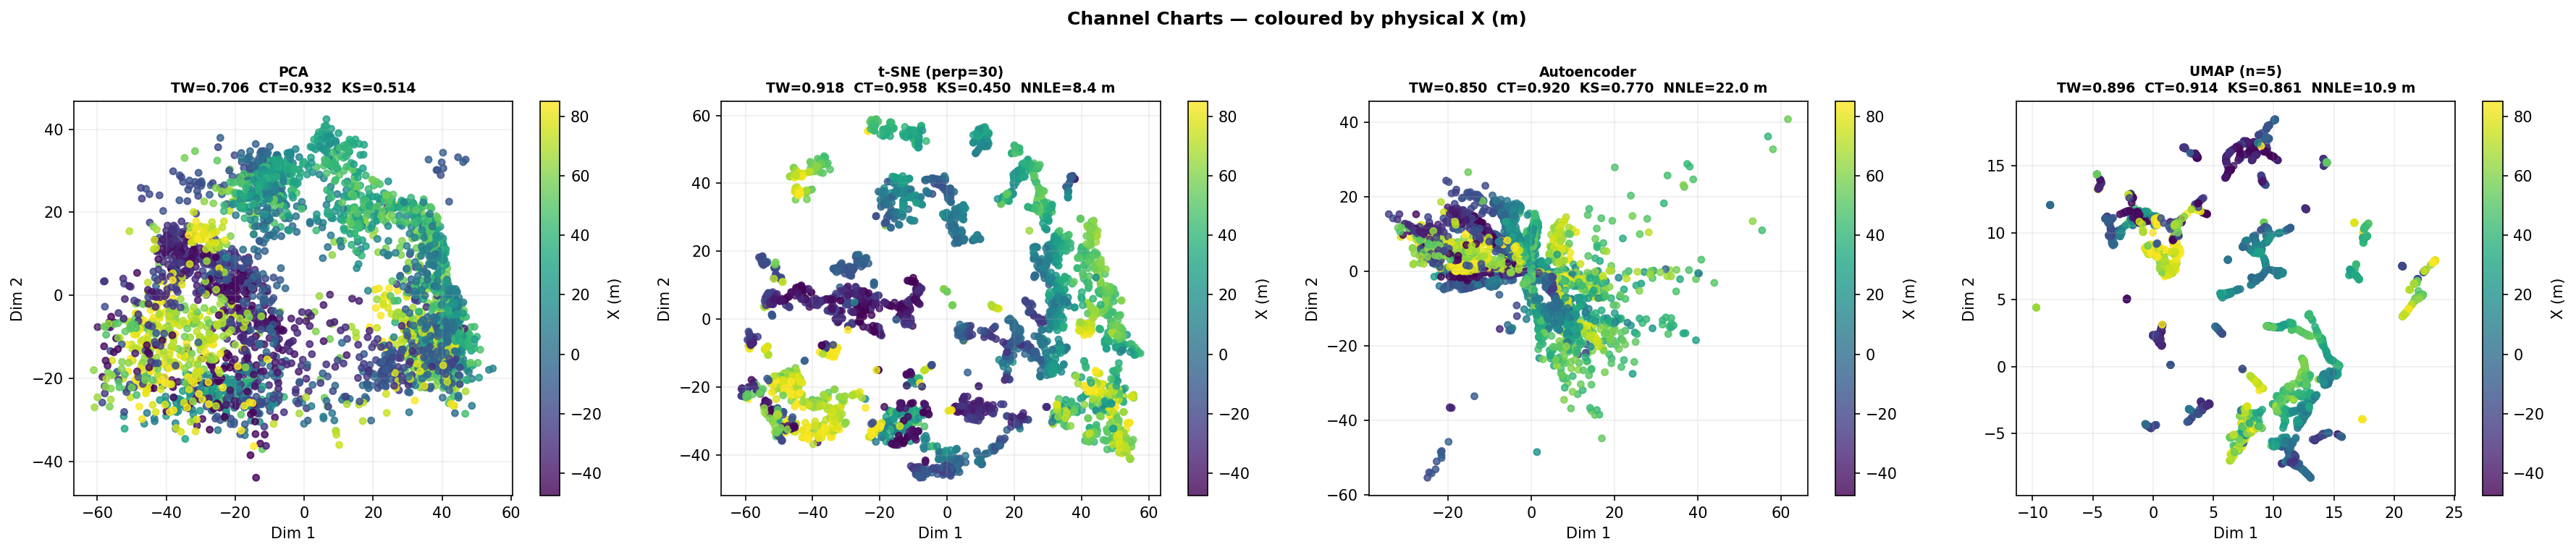
\includegraphics[width=\textwidth]{pictures/04_channel_charting/channel_charts_coloured_x.png}
  \caption{Channel charts produced by the four DR methods, coloured by
           the UE's ground-truth $x$ coordinate.  A smooth colour gradient
           indicates that the chart preserves one geographic axis.}
  \label{fig:cc_x}
\end{figure*}

\begin{figure*}[htbp]
  \centering
  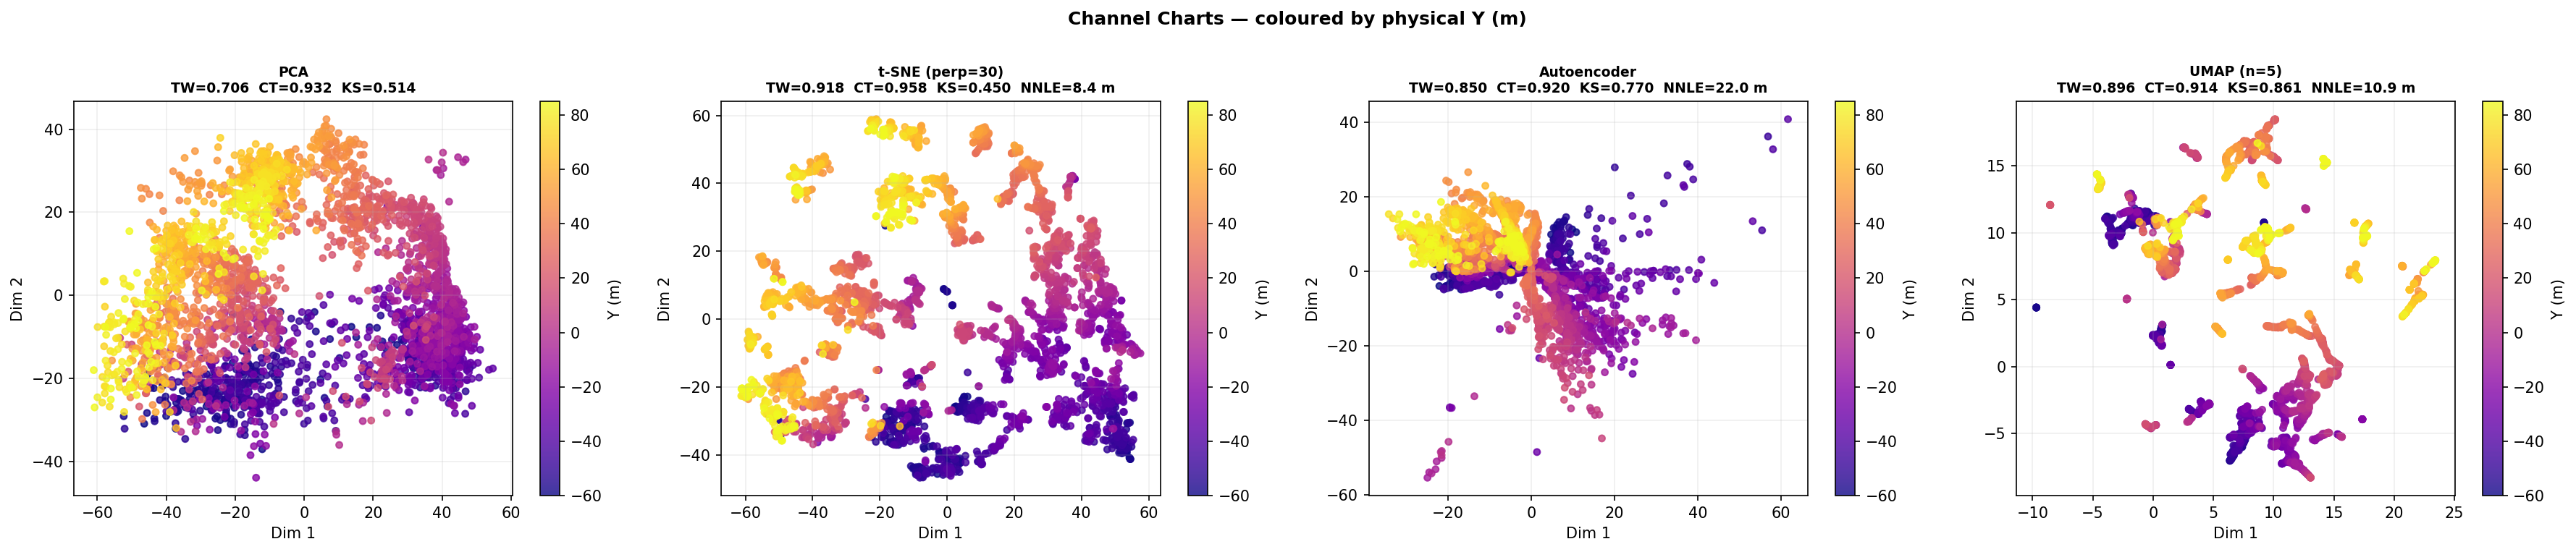
\includegraphics[width=\textwidth]{pictures/04_channel_charting/channel_charts_coloured_y.png}
  \caption{Same four charts coloured by the ground-truth $y$ coordinate.}
  \label{fig:cc_y}
\end{figure*}

\begin{figure*}[htbp]
  \centering
  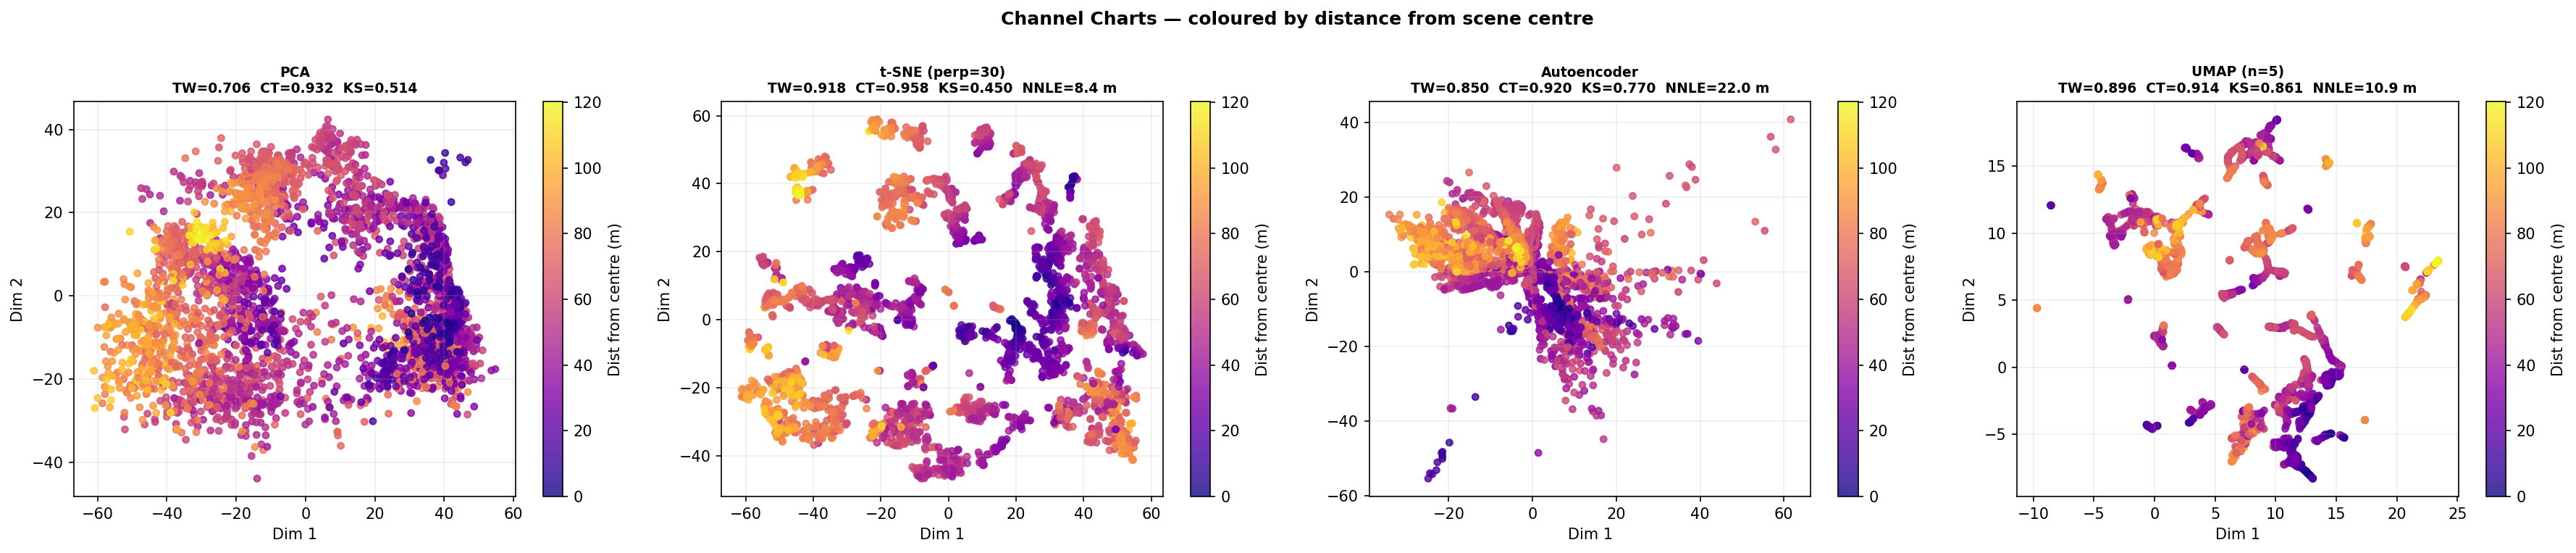
\includegraphics[width=\textwidth]{pictures/04_channel_charting/channel_charts_comparison.png}
  \caption{Charts coloured by distance from the scene centre.  t-SNE and
           UMAP produce the most geometrically consistent charts, PCA the
           most scale-faithful but topologically compressed one.}
  \label{fig:cc_comparison}
\end{figure*}

\begin{figure}[htbp]
  \centering
  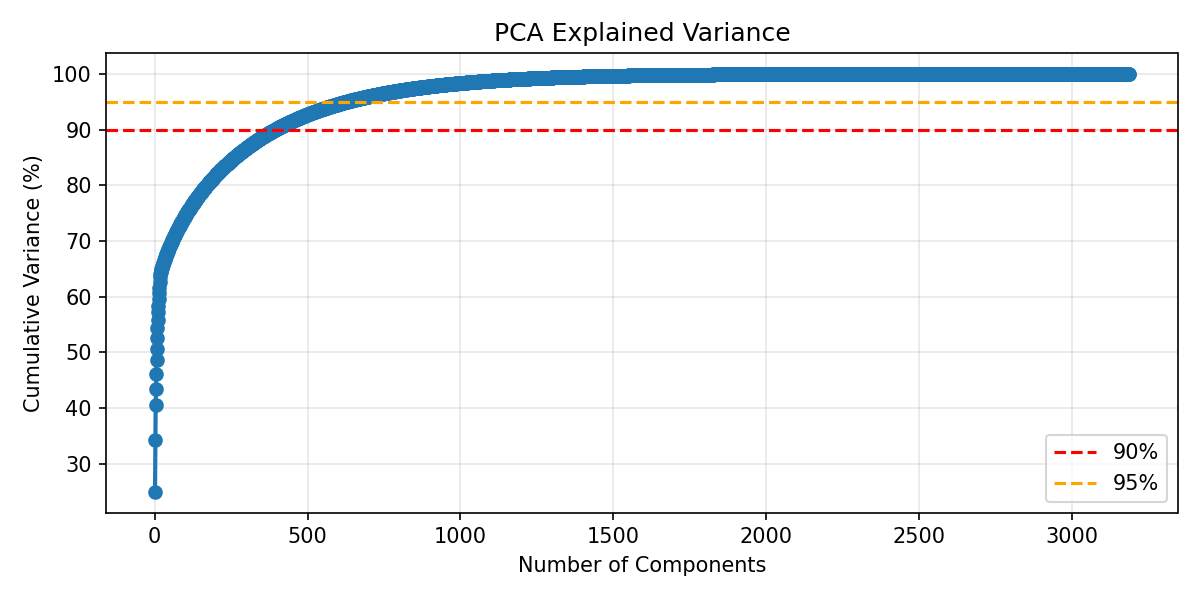
\includegraphics[width=\columnwidth]{pictures/04_channel_charting/pca_explained_variance.png}
  \caption{Cumulative explained variance of the PCA basis.  The first
           50 principal components, used as input to t-SNE and UMAP,
           capture the bulk of the fingerprint variance.}
  \label{fig:cc_pca}
\end{figure}

\subsection{Parameter Sensitivity}

Because t-SNE and UMAP are strongly sensitive to their local
neighbourhood parameters, both were swept on the same fingerprint matrix
(Table~\ref{tab:cc_sweep}).
t-SNE is relatively flat in TW for
$\text{perplexity}\in[15,50]$ but its KS score is minimised at
$\text{perplexity}=30$. Minum distance paramerter was set to 0.01 and 
metric was set to cosine for UMAP runs 
UMAP's $n_{\mathrm{neighbors}}$ trades neighbourhood TW against global
KS; the $n=5$ setting gives the best TW at the cost of a larger KS, and
is the working point reported in Table~\ref{tab:cc_metrics}.

\begin{table}[htbp]
\caption{Parameter sensitivity for t-SNE and UMAP}
\label{tab:cc_sweep}
\centering
\begin{tabular}{llrr}
\toprule
Method & Parameter                          & TW    & KS    \\
\midrule
t-SNE  & perplexity $= 5$                    & 0.906 & 0.459 \\
t-SNE  & perplexity $= 15$                   & 0.916 & 0.417 \\
t-SNE  & perplexity $= 30$                   & \textbf{0.918} & \textbf{0.450} \\
t-SNE  & perplexity $= 50$                   & 0.917 & 0.535 \\
\midrule
UMAP   & $n_{\mathrm{neighbors}} = 5$        & \textbf{0.896} & 0.861 \\
UMAP   & $n_{\mathrm{neighbors}} = 10$       & 0.896 & 0.870 \\
UMAP   & $n_{\mathrm{neighbors}} = 20$       & 0.895 & 0.884 \\
UMAP   & $n_{\mathrm{neighbors}} = 30$       & 0.891 & 0.898 \\
\bottomrule
\end{tabular}
\end{table}

\subsection{t-SNE and UMAP on MATLAB}

Table~\ref{tab:cc_sweep_matlab} summarises the performance of t-SNE and UMAP matlab
 implementations for different parameters and number of neighbors.  
 
 t-SNE perplexities are shown in Fig \ref{fig:cc_tsne_matlab}.



\begin{table}[htbp]
\caption{Parameter sensitivity for t-SNE and UMAP}
\label{tab:cc_sweep_matlab}
\centering
\begin{tabular}{llrrr}
\toprule
Method & Parameter                          & TW    & CT    &   KS\\
\midrule
t-SNE  & perplexity $= 30$                    & 0.8649 & 0.9024 & 0.4953\\
t-SNE  & perplexity $= 50$                    & 0.8515 &  0.9010 & 0.4847\\
t-SNE  & perplexity $= 100$                   & 0.8706 & 0.9007 & 0.4992\\
\midrule
UMAP   & $n_{\mathrm{neighbors}} = 5$        & 0.8618 & 0.8949 & 0.7451\\
UMAP   & $n_{\mathrm{neighbors}} = 10$       & 0.8769  & 0.8967 & 0.5509\\
UMAP   & $n_{\mathrm{neighbors}} = 20$       & 0.8771 & 0.8973 & 0.5771\\
UMAP   & $n_{\mathrm{neighbors}} = 30$       & 0.8472 & 0.8955 & 0.8049\\
\bottomrule
\end{tabular}
\end{table}


\begin{figure*}[htbp]
  \centering
  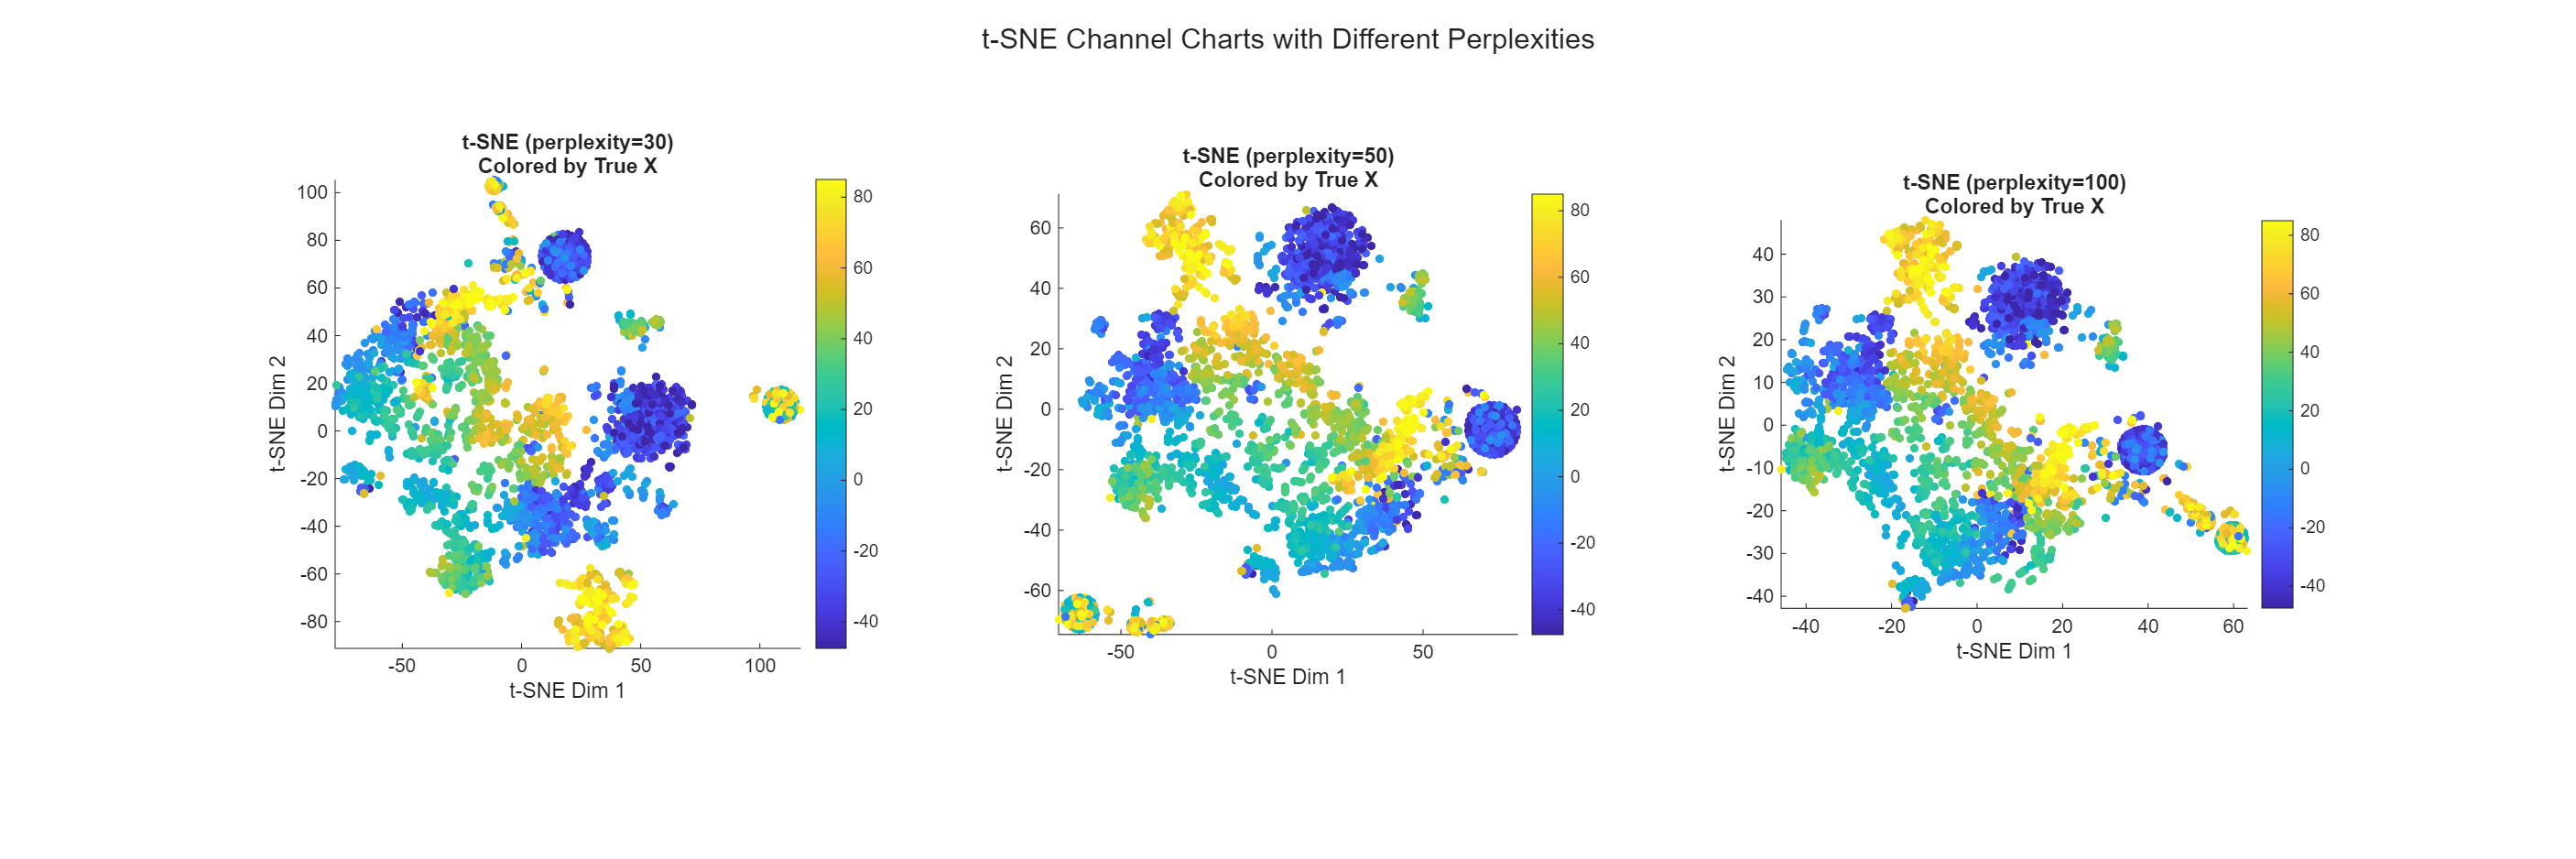
\includegraphics[width=\textwidth]{pictures/TSNE_perplexities.png}
  \caption{t-SNE channel charts for different perplexity values.}
  \label{fig:cc_tsne_matlab}
\end{figure*}



\subsection{Discussion}

t-SNE at perplexity $30$ is the best method on every metric, with
$\text{TW}=0.918$, $\text{CT}=0.958$, and a nearest-neighbour localisation
error of $8.35\,\text{m}$, which is on par with the best supervised
regressor of Section~\ref{sec:localization} despite using no UE labels.
UMAP trades a little TW/CT against substantially worse KS, which is the
expected behaviour of a method optimised for local topology preservation.
The autoencoder is the weakest of the four on KS ($0.77$) and NNLE
($22\,\text{m}$): its MSE reconstruction objective does not explicitly
encourage metric preservation in the latent space, and the small number
of training fingerprints ($N=3\,186$) is insufficient for a deep latent
model.
PCA, as expected, provides a cheap but strongly non-metric baseline
(high CT but poor TW and KS): variance directions in the CSI space are
not aligned with geographic axes.

Practical improvements fall into three categories:
\begin{enumerate}
  \item \emph{Richer fingerprints} --- include per-path AoA/AoD (already
        available in the HDF5 dataset) and stack CSI from all BSs
        equally rather than the current flat feature vector.
  \item \emph{Structure-aware losses} --- replacing the plain MSE
        autoencoder with a triplet or Siamese training
        objective~\cite{lei2019siamese_cc} would force the latent space
        to preserve neighbourhood relationships directly.
  \item \emph{Scene size} --- enlarging the UE grid (reducing
        \texttt{GRID\_SPACING}) increases the density of the fingerprint
        library and reduces the sampling noise in the DR metrics.
\end{enumerate}

\subsection{MATLAB Pipeline Cross-Check to Python environment}
\label{sec:matlab_channel_charting}

The same four DR methods were also applied to the MATLAB-derived
 fingerprints (Section~\ref{sec:matlab_dataset}),
with $N=3\,069$ UE positions and a much narrower feature vector
($D_f = 63$: AoA+RSS+Dly+Rch only).
Table~\ref{tab:cc_matlab} summarises the results.

\begin{table}[htbp]
\caption{Channel-charting metrics on the MATLAB tommiScene corpus ($N = 3\,069$, $D_f = 63$).  Best value per column in \textbf{bold}.}
\label{tab:cc_matlab}
\centering
\begin{tabular}{lrrrr}
\toprule
Method              & TW ($\uparrow$) & CT ($\uparrow$) & KS ($\downarrow$) & NNLE (m, $\downarrow$) \\
\midrule
PCA                 & 0.613            & 0.830            & 0.523              & n/a \\
t-SNE (perp.\ = 5)  & \textbf{0.975}   & \textbf{0.945}   & 6.828              & \textbf{19.46} \\
Autoencoder         & 0.754            & 0.885            & 0.478              & 40.02 \\
UMAP ($n=5$)        & 0.954            & 0.936            & \textbf{0.397}     & 22.04 \\
\bottomrule
\end{tabular}
\end{table}

Qualitatively the same ranking emerges as on the Sionna corpus: t-SNE
gives the best neighbourhood-preservation (highest TW, lowest NNLE),
UMAP is the best \emph{scale-faithful} chart (lowest KS), PCA is the
weak linear baseline, and the autoencoder struggles with the small
feature vector.
The absolute NNLE is worse than on the Sionna corpus
($19.46\,\text{m}$ vs.\ $8.35\,\text{m}$), consistent with the coarser
localization result in Section~\ref{sec:matlab_localization}: fewer
effective features means less neighbourhood information for the DR
method to exploit.
The MATLAB t-SNE KS value of $6.83$ is unusually large, reflecting the
fact that t-SNE's output is not globally scale-preserving; UMAP or PCA
are the right choices when absolute distance matters.

